% !TEX TS-program = pdflatex
% !TEX encoding = UTF-8 Unicode

% This is a simple template for a LaTeX document using the "article" class.
% See "book", "report", "letter" for other types of document.

\documentclass[11pt]{article} % use larger type; default would be 10pt

\usepackage[utf8]{inputenc} % set input encoding (not needed with XeLaTeX)

\usepackage{amsmath}

\usepackage{graphicx,url}
\usepackage{subfig}
\usepackage{multirow}

%%% Examples of Article customizations
% These packages are optional, depending whether you want the features they provide.
% See the LaTeX Companion or other references for full information.

%%% PAGE DIMENSIONS
\usepackage{geometry} % to change the page dimensions
\geometry{a4paper} % or letterpaper (US) or a5paper or....
% \geometry{margins=2in} % for example, change the margins to 2 inches all round
% \geometry{landscape} % set up the page for landscape
%   read geometry.pdf for detailed page layout information

\usepackage{graphicx} % support the \includegraphics command and options

% \usepackage[parfill]{parskip} % Activate to begin paragraphs with an empty line rather than an indent

%%% PACKAGES
\usepackage{booktabs} % for much better looking tables
\usepackage{array} % for better arrays (eg matrices) in maths
\usepackage{paralist} % very flexible & customisable lists (eg. enumerate/itemize, etc.)
\usepackage{verbatim} % adds environment for commenting out blocks of text & for better verbatim
\usepackage{subfig} % make it possible to include more than one captioned figure/table in a single float
% These packages are all incorporated in the memoir class to one degree or another...

%%% HEADERS & FOOTERS
\usepackage{fancyhdr} % This should be set AFTER setting up the page geometry
\pagestyle{fancy} % options: empty , plain , fancy
\renewcommand{\headrulewidth}{0pt} % customise the layout...
\lhead{}\chead{}\rhead{}
\lfoot{}\cfoot{\thepage}\rfoot{}

%%% SECTION TITLE APPEARANCE
\usepackage{sectsty}
\allsectionsfont{\sffamily\mdseries\upshape} % (See the fntguide.pdf for font help)
% (This matches ConTeXt defaults)

%%% ToC (table of contents) APPEARANCE
\usepackage[nottoc,notlof,notlot]{tocbibind} % Put the bibliography in the ToC
\usepackage[titles,subfigure]{tocloft} % Alter the style of the Table of Contents
\renewcommand{\cftsecfont}{\rmfamily\mdseries\upshape}
\renewcommand{\cftsecpagefont}{\rmfamily\mdseries\upshape} % No bold!

%%% END Article customizations

%%% The "real" document content comes below...

\title{Example to Accompany `A General, Parallel Implementation of Dantzig--Wolfe Decomposition'}
\author{Joseph Rios}
%\date{} % Activate to display a given date or no date (if empty),
         % otherwise the current date is printed 

\begin{document}
\maketitle

%----------------------------------------------------------------
%
%   Program options
%
%----------------------------------------------------------------
\section{Example}
\label{secOptions}
This note accompanies the article entitled ``A General, Parallel Implementation of Dantzig--Wolfe Decomposition'' submitted to and accepted for publication in ACM Transactions on Mathematical Software~\cite{RiosTOMS12}.  Here, I provide a simple example of how the software works, complete with input and output files.  The code is currently available at \url{http://sourceforge.net/projects/dwsolver}.

For this brief example, I will refer to the software by its command-line executable name:  dwsolver.  There are several user-supplied options available to dwsolver.  Currently there is no callable interface.  The program can print timing information, which includes the elapsed CPU time (the sum of all the seconds spent on all cores in the system) and elapsed wall clock time.  To aid in debugging models and tracing solution trajectories through the algorithm, several files may be written during the course of solving.  The basis may be output to a file at each iteration for the user to investigate how columns entered and exited the basis over the course of iterations.  In addition, the reduced master problem may be output to a file at each iteration.  After convergence upon an optimum value, the final reduced master problem can be saved to file.  Solving this final reduced master problem independently at any later time would provide the optimal solution to the original linear program.
%----------------------------------------------------------------
%
%   Examples
%
%----------------------------------------------------------------
%\section{Example}
%\label{secExamples}
As evidence of correctness and an aid in developing input files, several examples are provided with the software.  Most of the examples are taken directly from popular textbooks that discuss DW.  These include books from Bertsimas and Tsitsiklis~\cite{Bertsimas97}, Lasdon~\cite{Lasdon70}, and Dantzig~\cite{Dantzig63}.  There are also two examples from instructors' websites as well as a larger example taken from this author's work on air traffic management.

The best way to understand the input and output for the program is to look at a single example in its entirety.  For this purpose, Lasdon's example~\cite{Lasdon70} is used.  The original problem as given in the textbook is as follows:
\begin{align}
\text{minimize}& \quad z =& -&x_1 &- &x_2& - &2y_1 &- &y_2 \nonumber \\
\text{subject to}& \quad& &x_1 &+ &2x_2 &+&2y_1& +& y_2 &\le 40 \label{eqnExConnecting}\\
&&&x_1 &+ &3x_2&&&&&\le30 \label{eqnExSub1a}\\
&&&2x_1 &+ &x_2&&&&&\le20 \label{eqnExSub1b}\\
&&&&&&&y_1&&&\le10\label{eqnExSub2a} \\
&&&&&&&&&y_2&\le10 \label{eqnExSub2b}\\
&&&&&&&y_1&+&y_2&\le15 \label{eqnExSub2c}
\end{align}

Inequality~\ref{eqnExConnecting} will be the sole connecting constraint, while Inequalities~\ref{eqnExSub1a} and~\ref{eqnExSub1b} will form subproblem one and Inequalities~\ref{eqnExSub2a},~\ref{eqnExSub2b}, and~\ref{eqnExSub2c}~will form subproblem two.  Given this decomposition, the input files written in CPLEX's LP format~\cite{cplexmanual} are provided in Figure~\ref{figSubprobs}.  Note that in CPLEX's LP format, coefficients of unit value may be omitted and a sign on a coefficient may or may not be spaced from the coefficient.  Including spacing as shown in Figure~\ref{figSubprobs} is a convention often used to maintain spacing regularity in a text file.
%{\footnotesize
%\begin{verbatim}
%Minimize
% objective: - 1 x1 - 1 x2 - 2 y1 - 1 y2
%
%Subject To
% Con1: 1 x1 + 2 x2 + 2 y1 + 1 y2 <= 40
%
%end 
%\end{verbatim}
%}
%The first subproblem file:
%{\footnotesize
%\begin{verbatim}
%Minimize
% objective: - 1 x1 - 1 x2
% 
%Subject to
% c1: x1   + 3 x2 <= 30
% c2: 2 x1 + 1 x2 <= 20
%
%end
%\end{verbatim}
%}
%Finally, the second subproblem file:
%{\footnotesize
%\begin{verbatim}
%Minimize
% objective: - 2 y1 - 1 y2
% 
%Subject to
% c1: 1 y1        <= 10
% c2:        1 y2 <= 10
% c3: 1 y1 + 1 y2 <= 15
%
%end
%\end{verbatim}
%}
\begin{figure}
  \centering              
  \subfloat[Subproblem 1]{\label{figSub1}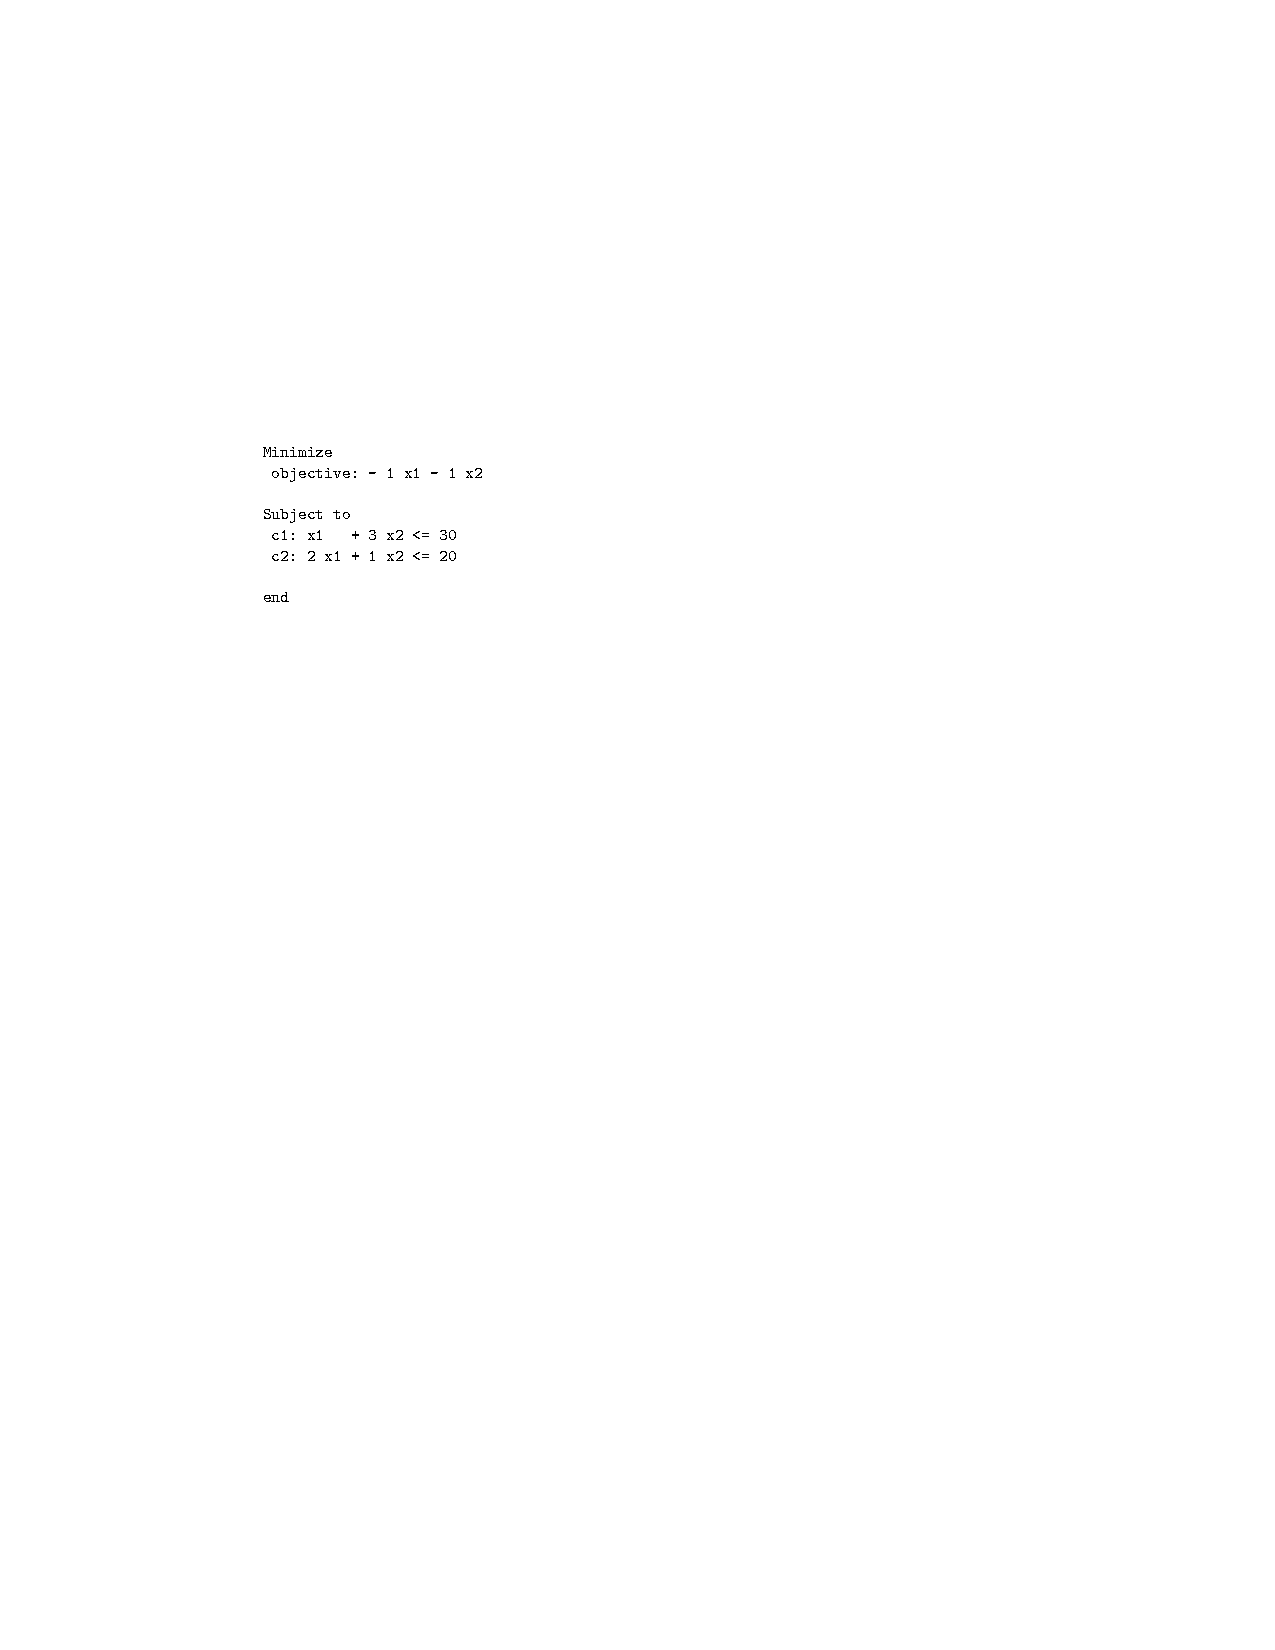
\includegraphics[width=0.4\textwidth]{sub1.pdf}}
  \hspace{0.5in}
  \subfloat[Subproblem 2]{\label{figSub2}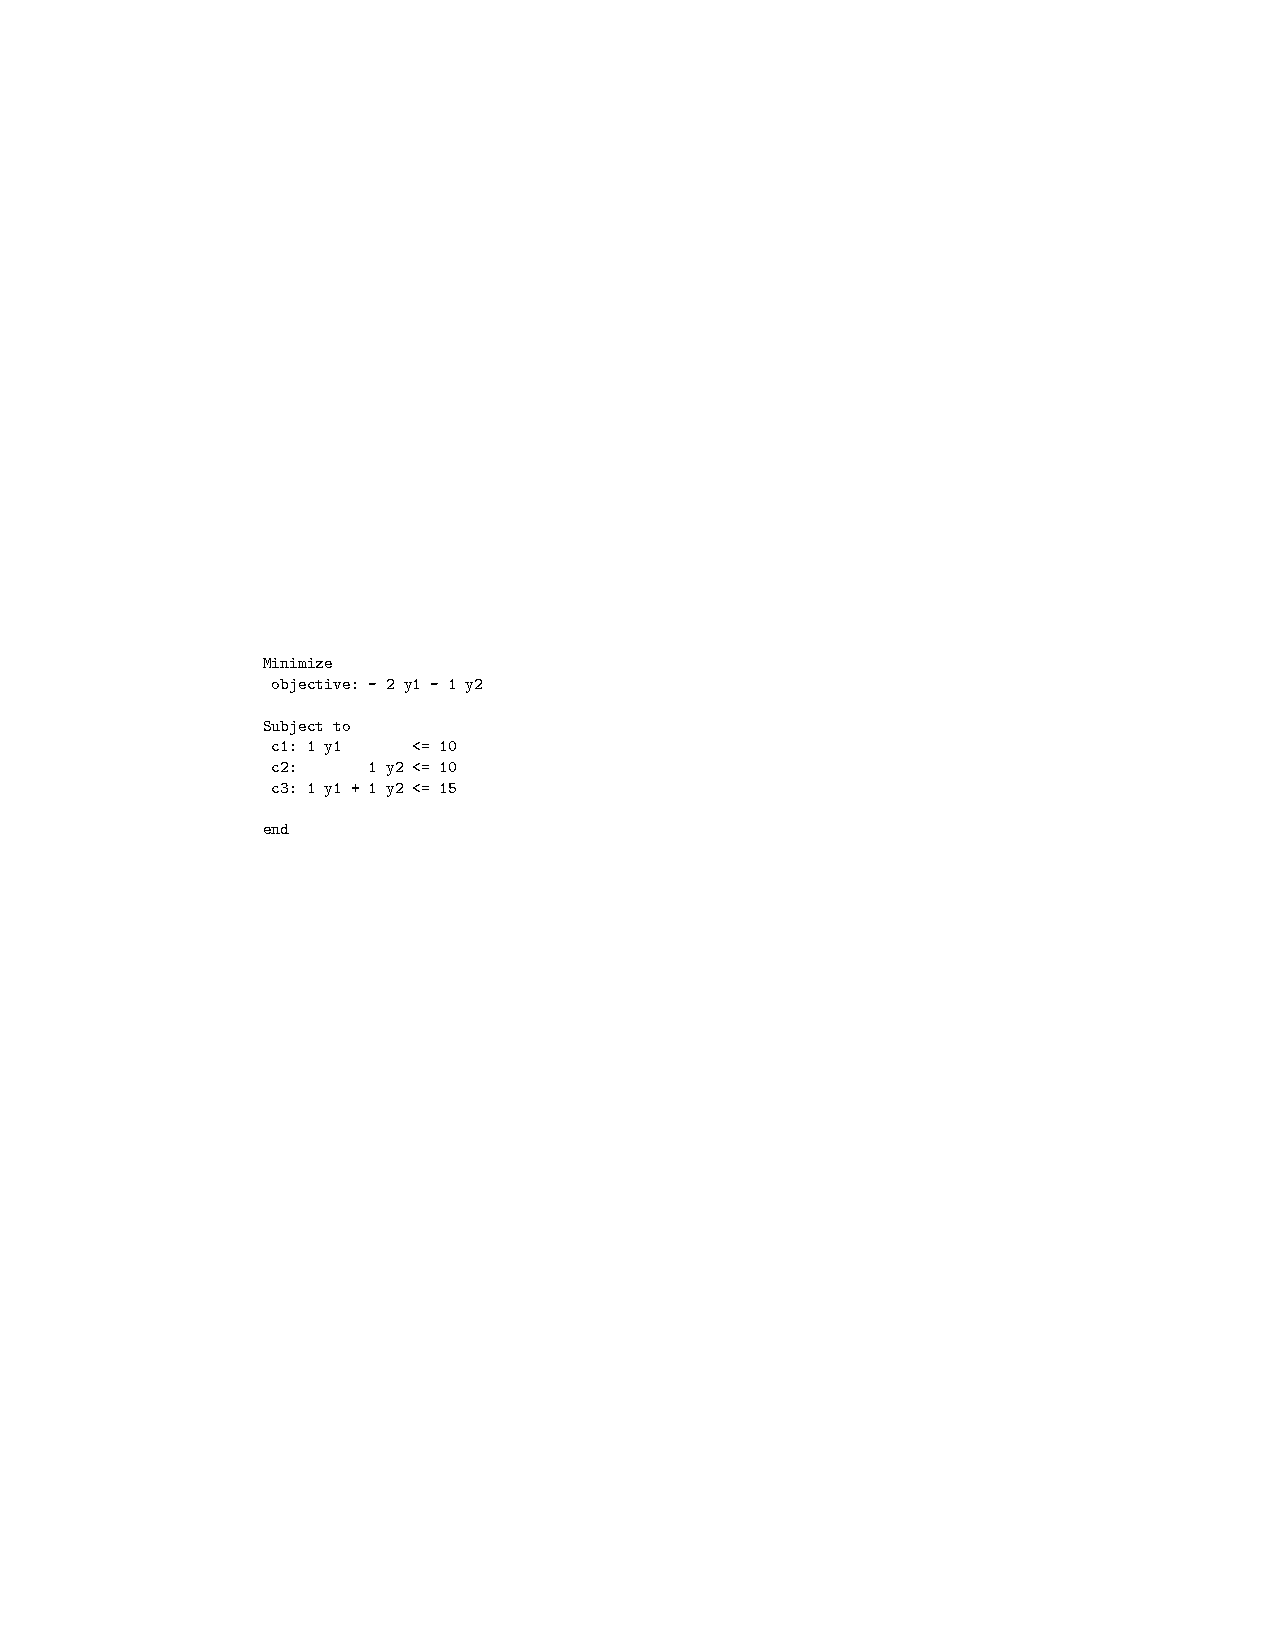
\includegraphics[width=0.38\textwidth]{sub2.pdf}}
   \hspace{0.5in}
  \subfloat[Master Problem]{\label{figMasterProb}  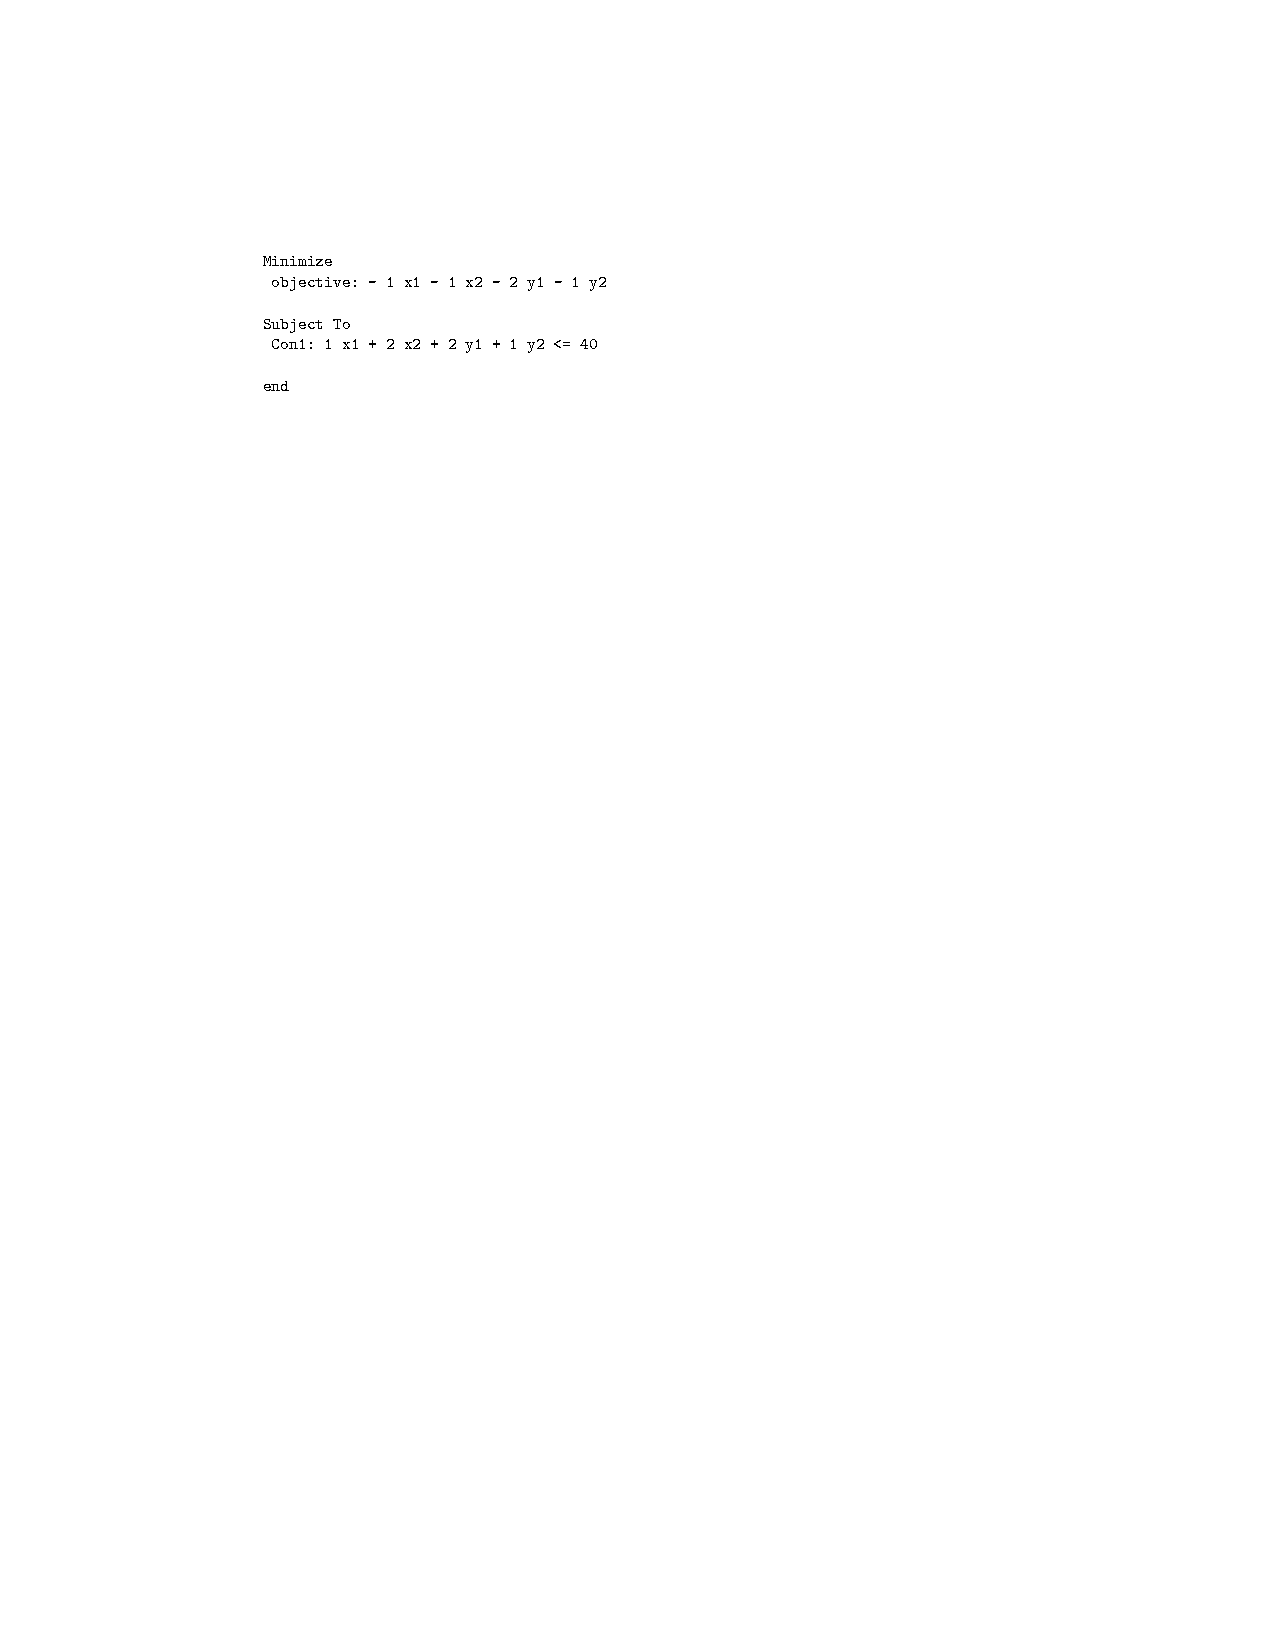
\includegraphics[width=0.6\textwidth]{master.pdf}}
  \caption{The two subproblems and master problem for the Lasdon example in LP format.}
 % \caption{The master problem for the Lasdon example in LP format.}
  \label{figSubprobs}
\end{figure}
Since dwsolver is a command-line tool and there may be many more than two subproblems, a guide file is used to declare these input files to dwsolver.  This guide file tells the program how many subproblem files there are, the names of each subproblem file, the name of the master file, and an optional, signed constant to be added to the objective value.  For this example, the guide file is implemented as shown in Figure~\ref{figGuideFile}.
\begin{figure}
\begin{center}
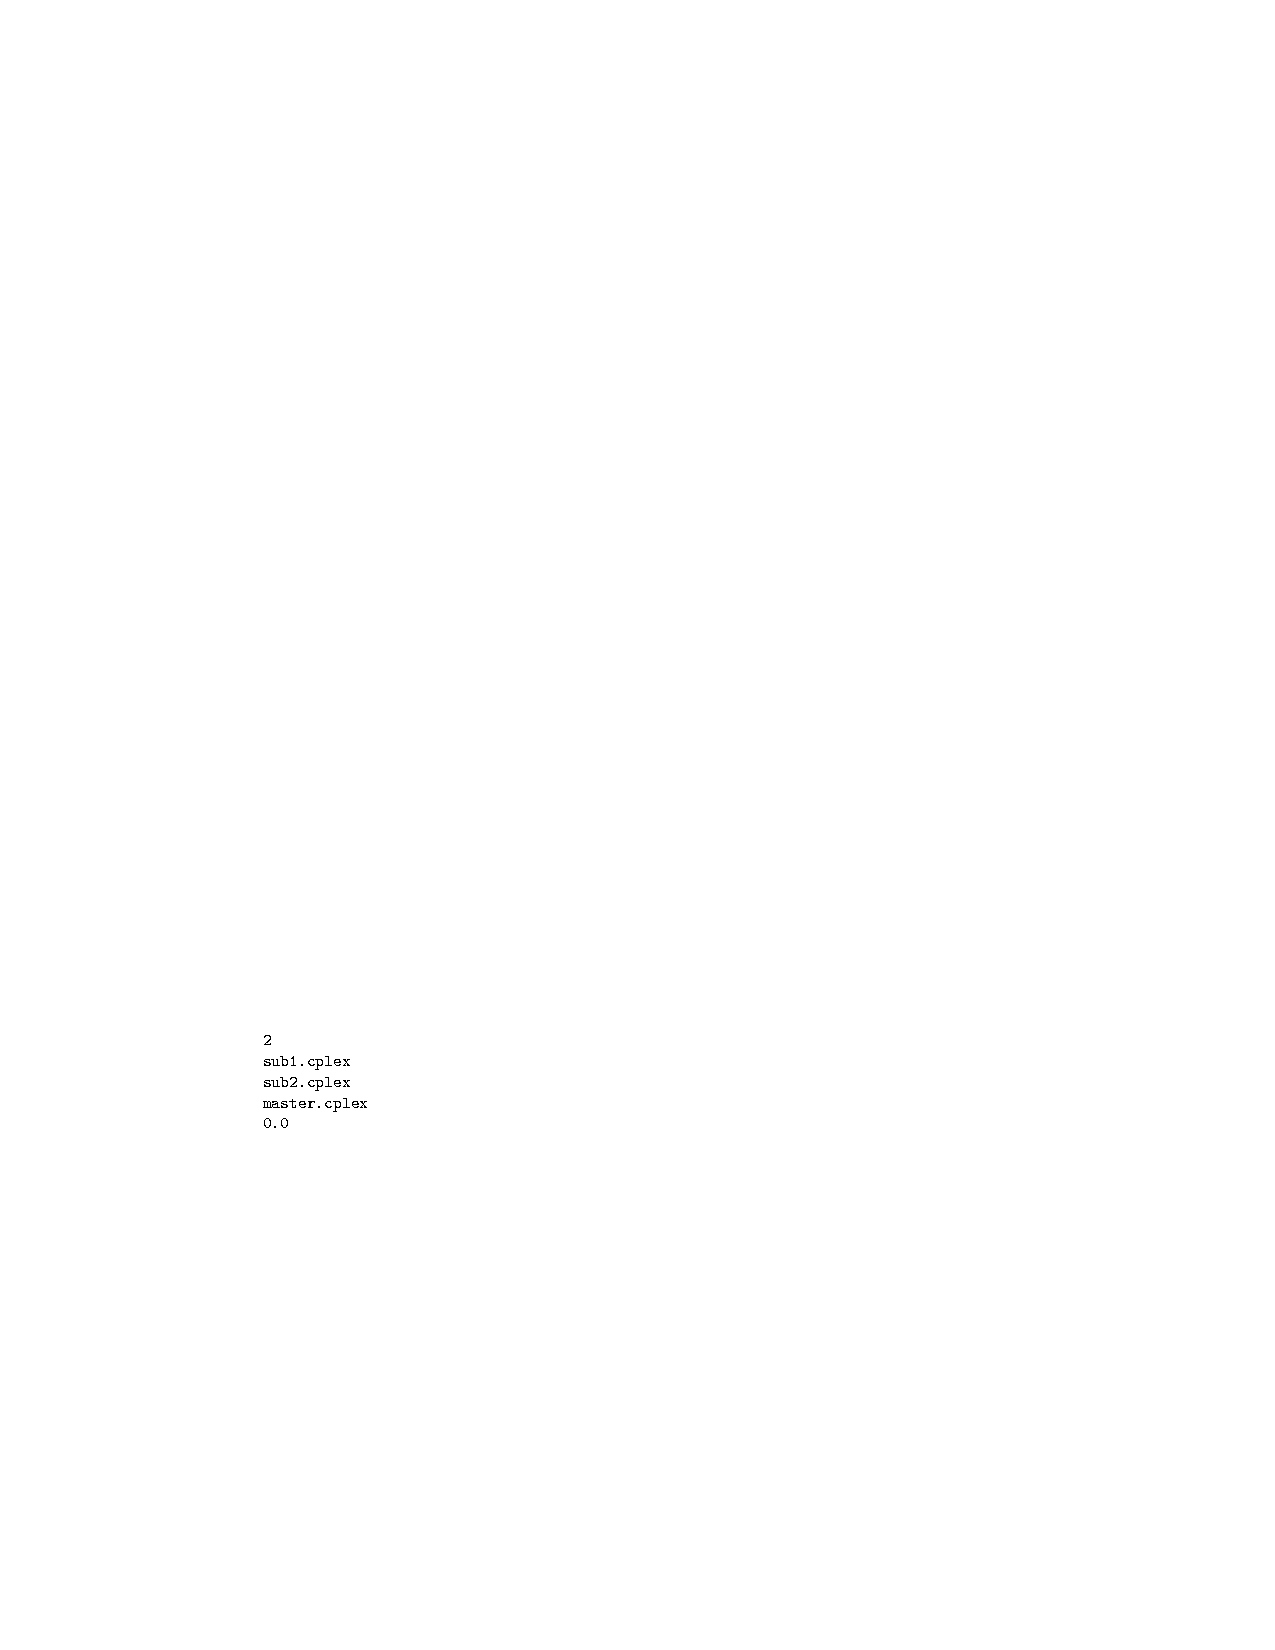
\includegraphics[width=0.22\textwidth]{guideFile.pdf}
 \caption{\label{figGuideFile} The Lasdon example guide file provided to {\tt dwsolver} with number of subproblems, subproblem file names, master file name, and objective constant value.}
 \end{center}
\end{figure}

Given these files, the command line ``{\tt dwsolver -g guide\_file}'' produces the terminal output shown in Figure~\ref{figTerminal} along with the solution file shown in Figure~\ref{figSolution}, which provides a mapping of variable names to value assignments for the discovered optimal value.  The optimal solution ($-36 \frac{2}{3}$) and the accompanying variable assignments are equal to those provided by Lasdon~\cite{Lasdon70}.
\begin{figure}[h!]
\begin{center}
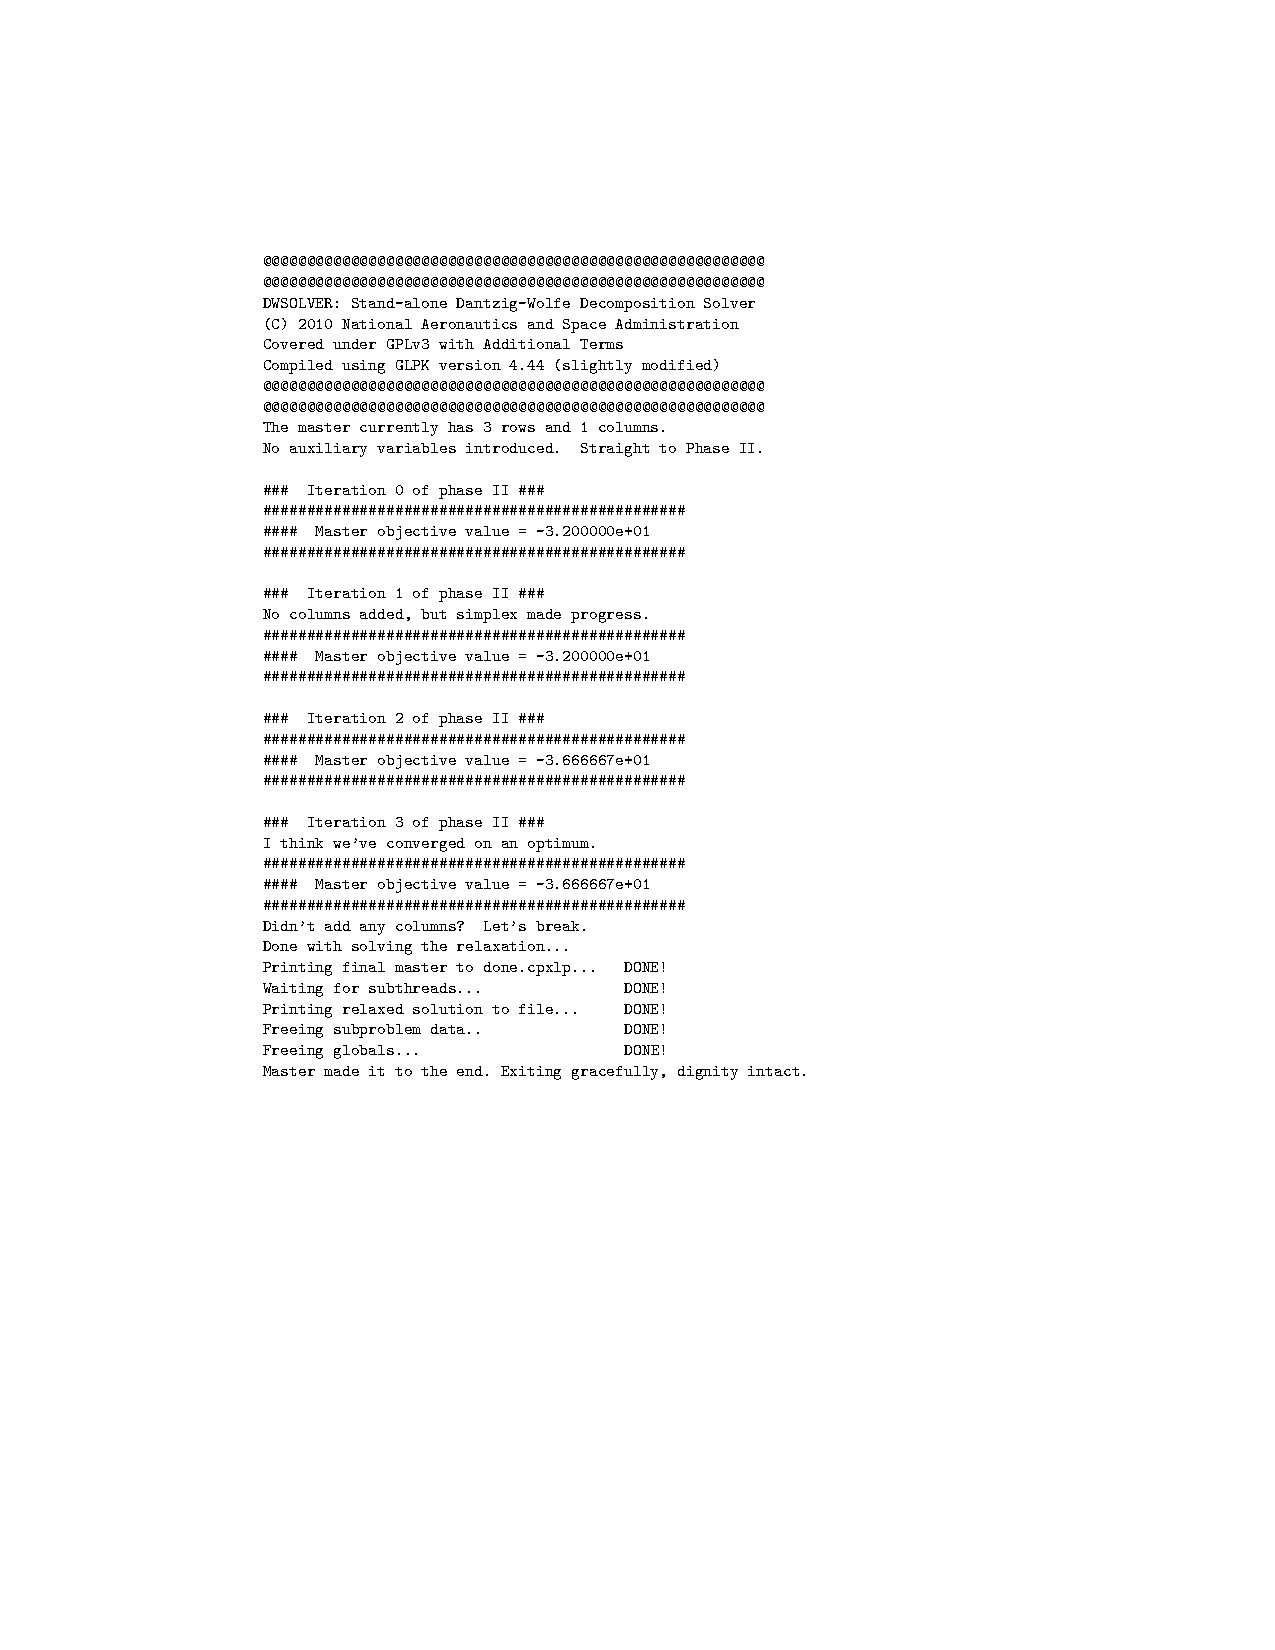
\includegraphics[width=0.7\textwidth]{exampleOutput.pdf}
 \caption{\label{figTerminal} Example terminal output from {\tt dwsolver} for the Lasdon example.}
 \end{center}
\end{figure}
\begin{figure}[h!]
\begin{center}
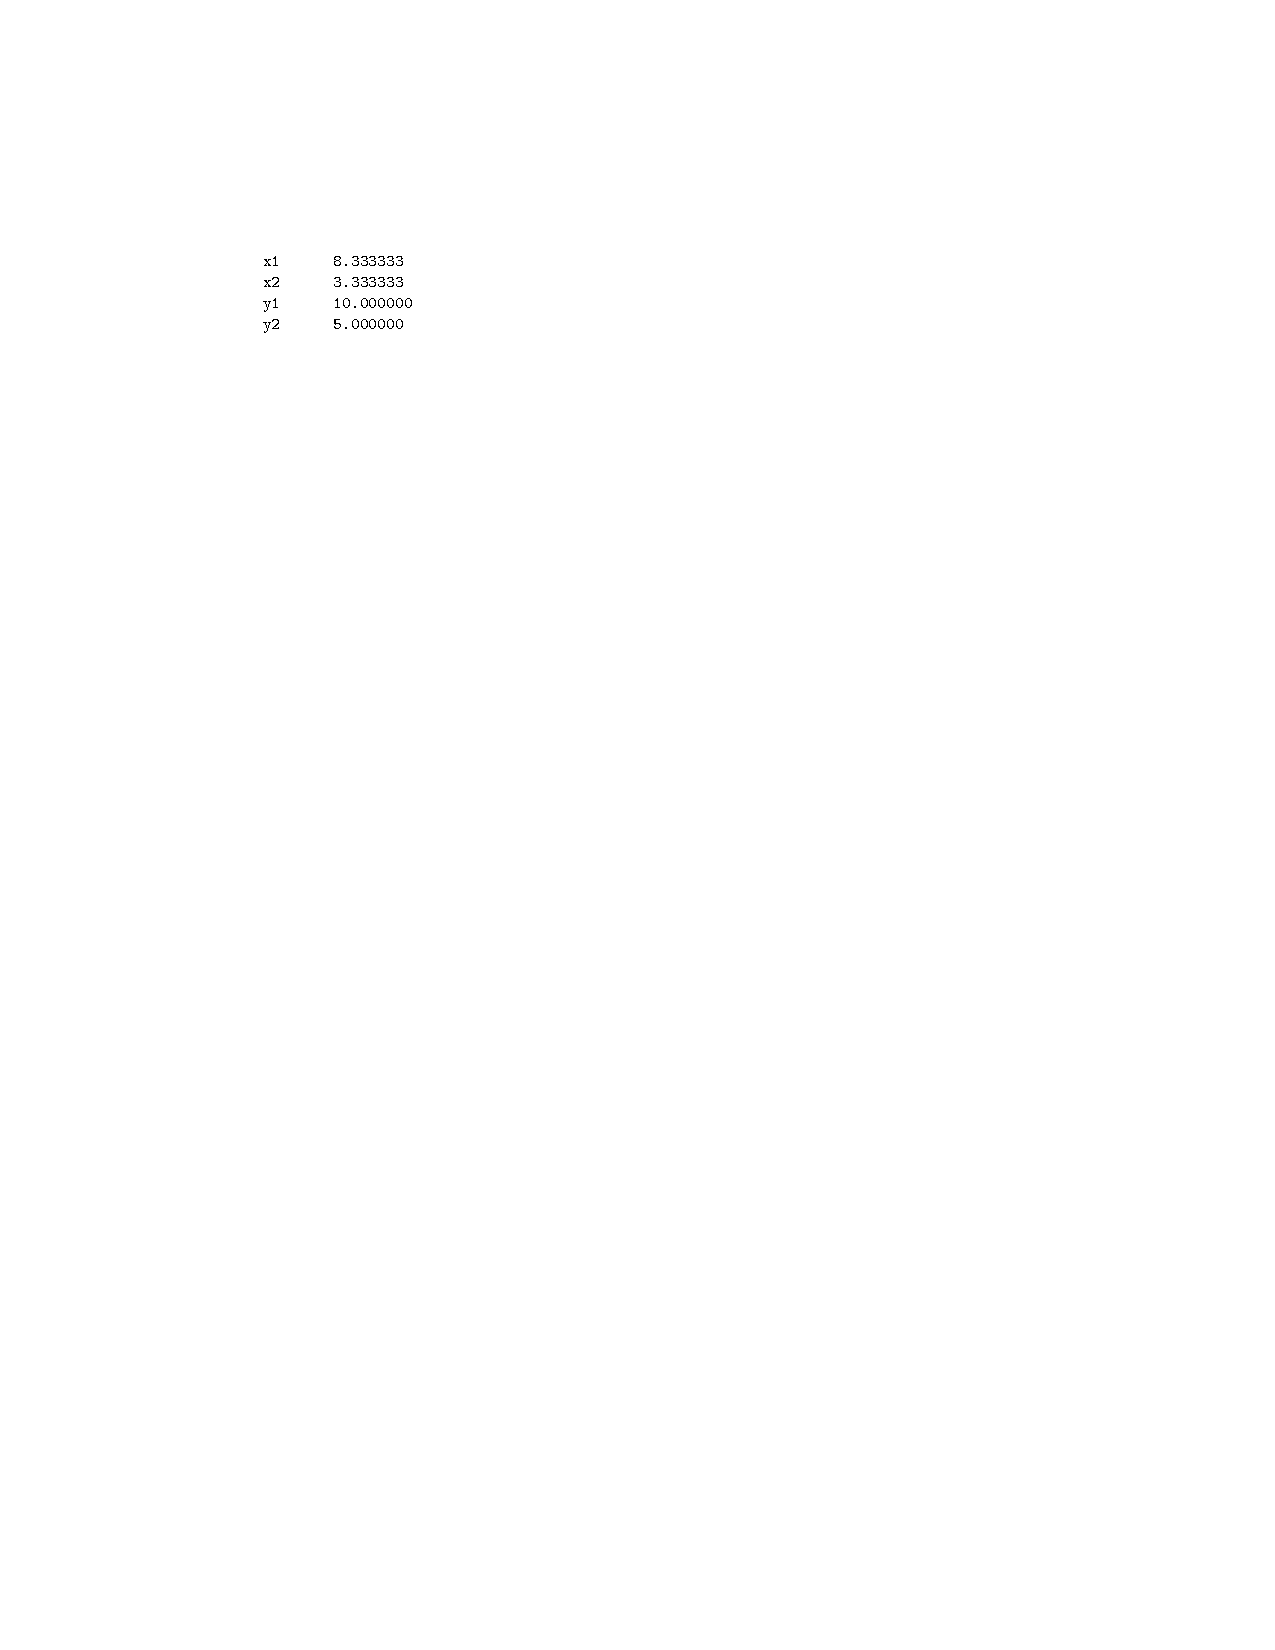
\includegraphics[width=0.25\textwidth]{solution.pdf}
 \caption{\label{figSolution} Example solution file from {\tt dwsolver} for the Lasdon example.}
 \end{center}
\end{figure}
\clearpage
\bibliographystyle{plain}
\bibliography{dw_software}

\end{document}
